\section{Method}

\subsection{Environments}

\begin{frame}
    \frametitle{Environments}
    
    \begin{itemize}
        \item Three simulated environments.
        % following the problem statement
        % gives control over difficulty to solve
        % more investigative power
        \item Find three targets in less than 1 000 steps.
        % otherwise unsuccessful
        \item There is some structure that can be utilized to find targets quicker.
        %\item Target probability correlated with scene appearance. 
        % possible to do better than exhaustive search on average
        % at least for a human
        \item Procedurally generated, conditioned on seed.
        % seed determines scene appearance and target positions
        % every scene slightly different
        % find common characteristics across seeds
        % can vary number of scenes by limiting seed pool
        \item New seed after each finished search.
    \end{itemize}
\end{frame}

\begin{frame}
    \frametitle{Observation, Action and Reward}

    \begin{itemize}
        \item Observations \(o_t = \left\langle x_t, p_t \right\rangle\), where
        \begin{itemize}
            \item \(x_t \in \mathbb{R}^{3 \times 64 \times 64}\) is an RGB image,
            \item \(p_t \in \{0, \dots, H\} \times \{0, \dots, W\}\) is the camera position.
        \end{itemize}
        \item Actions \(a_t \in \{\texttt{INDICATE}, \texttt{UP}, \texttt{DOWN}, \texttt{LEFT}, \texttt{RIGHT}\}\), where
        \begin{itemize}
            \item \texttt{INDICATE} identifies targets, and
            \item \texttt{UP}, \texttt{DOWN}, \texttt{LEFT}, \texttt{RIGHT} move camera.
        \end{itemize}
        \item Reward \(r_t = h - 0.01 + 0.005d + 0.005e\) where
        % in general, reward turned out to be tricky thing.
        % in our case, it was a design parameter
        % should achieve the goal of minimizing search time
        % small changes in magnitude let to drastically different results
        \begin{itemize}
            \item \(h = \left\vert T \cap V \right\vert\) if \(a_t = \texttt{INDICATE}\), else \(0\).
            % rewarded for finding targets
            % time penalty ensures that agent prioritizes finding targets quickly, as future reward is maximized when time is minimized.
            \item \(d = 1\) if \(a_t\) moves closer to nearest target, else \(0\).
            % rewarded for moving towards targets
            % not optimal, as greedily moving towards nearest target does not always yield an optimal travel path
            % however, not realistic in partially observable environments
            % experimentation showed that this term helped learning in difficult environments
            \item \(e = 1\) if \(a_t\) moves to new position, else \(0\).
            % always good to explore environment
            % important that it is not better than finding targets quickly!
        \end{itemize}
    \end{itemize}
\end{frame}

\begin{frame}
    \frametitle{Environment I: Gaussian}
    \begin{columns}
        \begin{column}{0.5\textwidth}
            \begin{itemize}
                % explain better, avoid using math description
                \item Three gaussian kernels with random center.
                \item Sum of three gaussian kernels = blue color intensity.
                \item More blue \rightarrow higher target probability.
                \item Agent should prioritize blue regions.
            \end{itemize}
        \end{column}
        \begin{column}{0.5\textwidth}
            \begin{figure}
                \centering
                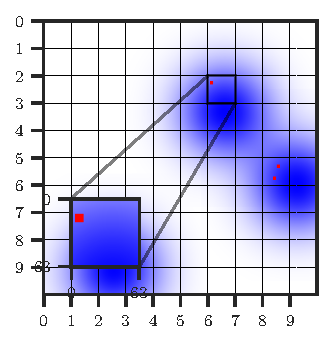
\includegraphics[scale=1.0]{figures/gaussian.pdf}
            \end{figure}
        \end{column}
    \end{columns}    
\end{frame}

\begin{frame}
    \frametitle{Environment II: Terrain}
    \begin{columns}
        \begin{column}{0.5\textwidth}
            \begin{itemize}
                \item Terrain seen from above (e.g. UAV).
                \item Targets between ocean and mountains.
                \item More realistic, higher variance.
            \end{itemize}
        \end{column}
        \begin{column}{0.5\textwidth}
            \begin{figure}
                \centering
                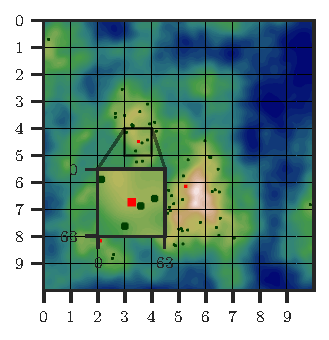
\includegraphics[scale=1.0]{figures/terrain.pdf}
            \end{figure}
        \end{column}
    \end{columns}   
\end{frame}

\begin{frame}
    \frametitle{Environment III: Camera}
    \begin{columns}
        \begin{column}{0.5\textwidth}
            \begin{itemize}
                \item Terrain seen from perspective projection camera.
                \item Variance in target appearance.
                \item Moving actions control pan and tilt.
                \begin{itemize}
                    \item 20 pan angle steps.
                    \item 10 tilt angle steps.
                \end{itemize}
            \end{itemize}

            \begin{figure}
                \centering
                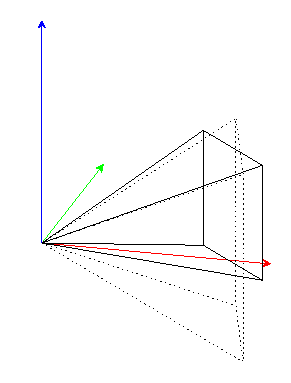
\includegraphics[scale=1]{figures/perspective.pdf}
            \end{figure}
        \end{column}
        \begin{column}{0.5\textwidth}
            \begin{figure}
                \centering
                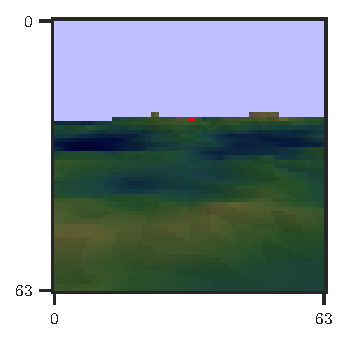
\includegraphics[scale=1.0]{figures/camera.pdf}
            \end{figure}
        \end{column}
    \end{columns}
\end{frame}

\subsection{Approach}

\begin{frame}
    \frametitle{Approach}

    \begin{itemize}
        \item Function approximation with deep neural networks.
        \begin{itemize}
            \item Policy \(\pi(a | s, \theta)\).
            \item Value \(v_\pi(s, \theta)\) (predicts future reward).
        \end{itemize}
        \item Training procedure:
        \begin{enumerate}
            \item Collect interactions with environment.
            \item Compute loss \(\mathcal{L(\theta)}\).
            \item Optimize \(\mathcal{L}\) wrt \(\theta\).
            \item Repeat until \(\pi\) is good.
        \end{enumerate}
        \item Use proximal policy optimization~\cite{schulman_proximal_2017}.
        \begin{itemize}
            \item RL algorithm from 2017.
            \item Stable performance, relatively little tuning~\cite{henderson_deep_2018}.
        \end{itemize}

    \end{itemize}
\end{frame}

\begin{frame}
    \frametitle{Architecture}

    \begin{figure}
        \centering
        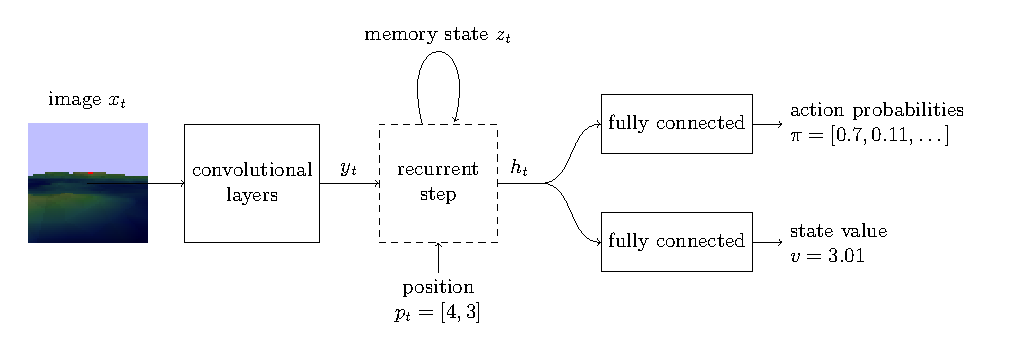
\includegraphics[scale=0.75]{figures/architecture-visual.pdf}
    \end{figure}

\end{frame}

\begin{frame}
    \frametitle{Memory}

    \begin{itemize}
        \item \textit{Agent should remember visual features and associate them with their spatial location.}
        % this is a hypothesis.
        % should be useful for visual search in the general case.
        % make decisions based on whole explored scene so far.
        % best action depends on history of interactions
        \item Two memory variants:
        \begin{enumerate}
            \item Temporal memory (long short-term memory~\cite{hochreiter_long_1997}):
            \begin{itemize}
                \item Previously applied successfully to tasks where memory is required~\cite{hausknecht_deep_2017,mnih_asynchronous_2016}.
                \item How long sequences can be remembered?
                % Can be important for exhaustive search and scene understanding.
                % Can it reason over spatial relationships?
            \end{itemize}
            \item Spatial memory (inspired by \cite{parisotto_neural_2017} and \cite{gupta_cognitive_2019}):
            \begin{itemize}
                \item Feature map with one slot per camera position.
                \item Indexed with current position.
                \item Stores image representation at each slot.
                \item Read whole memory with convolutional layers.
                % Visualization of the memory comes later.
            \end{itemize}
        \end{enumerate}
    \end{itemize}
\end{frame}

\begin{frame}
    \frametitle{Training}

    \begin{itemize}
        \item Train for 25M time steps.
        % This was sufficient for convergence in each environment.
        \item Results reported across 3 training runs.
        % Deep RL known to have reproducibility problem.
        % This is a widely discussed topic.
        % Different runs have been shown to yield learning curves from different distributions.
        % Important to do multiple runs to get a sense of stability
        % We report mean and standard deviation.
        \item Separate training and test sets.
        % Ensures that agents do not simply memorize certain scenarios.
        %\item Same hyperparameters in all runs.
        % Training takes long time
        % (deep RL is sample-inefficient)
        % This means that extensive hyperparameter tuning is not an option
        % (unless sufficient compute resources available)
    \end{itemize}
\end{frame}

\begin{frame}
    \frametitle{Implementation}

    \begin{itemize}
        \item OpenAI Gym environment interface.
        \item Custom proximal policy optimization implementation.
        \item PyTorch for models and automatic differentiation.
        \item Intel Core i9-10900X CPU.
        \item NVIDIA GeForce RTX 2080 Ti GPU.
    \end{itemize}
\end{frame}